\chapter{实验结果与性能分析}


%*********************************************************************
% 5.1 全局指令选择正确性验证
%*********************************************************************
\section{全局指令选择正确性验}
本节通过一组具有代表性的LLVM IR示例程序,对DSP架构下的基于GlobalISel框架的代码生成流程进行正确性验证。验证重点覆盖LLVM IR向GMIR的转换、指令合法化、寄存器组选择以及机器指令选择这四个主要阶段。通过对关键Pass阶段的中间结果进行对比分析,系统性地验证全局指令选择流程在DSP后端中的功能正确性与稳定性。


% 5.1.1 基本指令正确性验证
\subsection{基本指令正确性验证}
本节旨在验证DSP后端基本指令的正确性,重点关注算术运算指令与内存访问指令的指令选择结果。为此,本文构造了一个综合示例一,该示例同时包含函数参数传递、内存读写操作以及整数加法与乘法运算等典型计算模式,能够覆盖DSP后端中最常见的指令选择路径。

\par

由于LLVM IR具有良好的目标无关性,且从C语言到LLVM IR的转换过程并非本文关注重点,本文在分析过程中省略前端生成IR的具体细节,直接展示从LLVM IR到目标机器码的转换流程,以突出指令选择与后端代码生成阶段的行为特征。

1.LLVM IR输入

示例一的LLVM IR如下所示(已去除调试信息):

\lstset{language=c++}
\begin{lstlisting}
define dso_local i32 @testArith(i32 noundef %a, i32 noundef %b) {
	entry:
	%a.addr = alloca i32
	%b.addr = alloca i32
	store i32 %a, ptr %a.addr
	store i32 %b, ptr %b.addr
	%0 = load i32, ptr %a.addr
	%1 = load i32, ptr %b.addr
	%add = add i32 %0, %1
	%2 = load i32, ptr %a.addr
	%mul = mul i32 %add, %2
	ret i32 %mul
}
\end{lstlisting}

2.GMIR生成阶段

如图\ref{fig:case_1_gmir_gen_dump}所示,在GMIR生成阶段,LLVM IR被转换为与目标架构无关的GMIR。从IR Dump的结果可以观察到:

\begin{itemize}
	\item
	add与mul指令分别被映射为G\_ADD与G\_MUL;
	
	\item
	load与store被转换为G\_LOAD与G\_STORE;
	
	\item 
	函数参数通过COPY指令从物理寄存器拷贝到虚拟寄存器。
	
\end{itemize}

\begin{figure}[htbp]
	\centering
	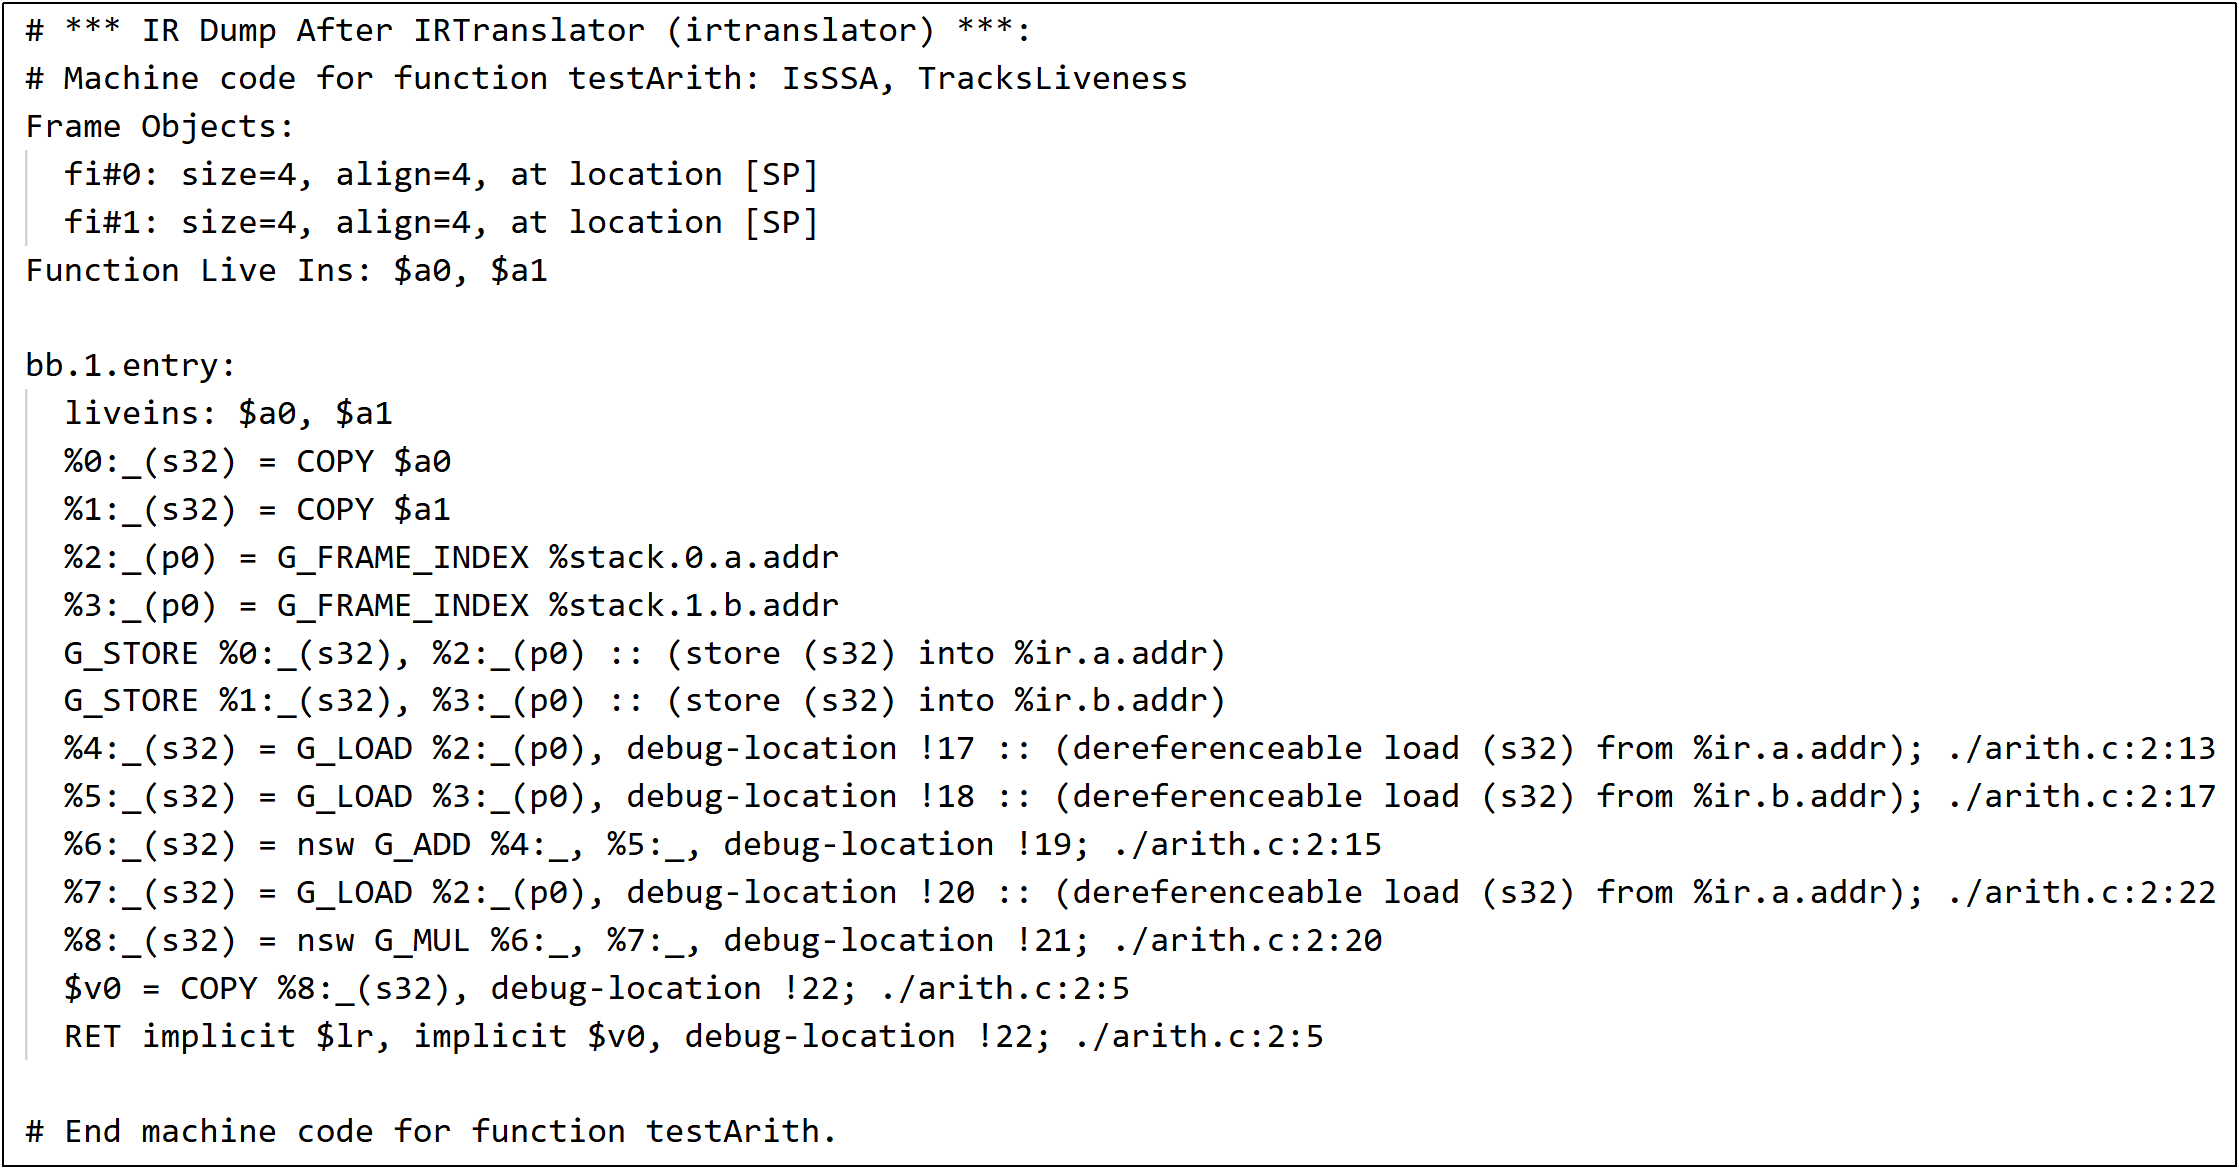
\includegraphics[width=1\textwidth]{pics/case_1_gmir_gen_dump.png}
	\caption{示例一GMIR生成阶段Dump图}
	\label{fig:case_1_gmir_gen_dump}
\end{figure}

该结果表明,LLVM IR到GMIR的转换过程保持了原有运算语义与数据依赖关系,为后续后端处理提供了正确的输入。

3.合法化阶段

合法化阶段的主要任务是将GMIR中不被目标架构直接支持的指令形式,转换为目标架构可处理的合法形式。由于32bit的G\_ADD、G\_MUL、G\_LOAD和G\_STORE指令在DSP架构下均为合法操作,于是示例中并未触发类型扩展、分裂或指令拆分等复杂合法化操作。如图\ref{fig:case_1_legalize_dump}所示,合法化前后指令结构保持一致,说明DSP的合法化规则能够正确覆盖基本算术与内存访问指令。

\begin{figure}[htbp]
	\centering
	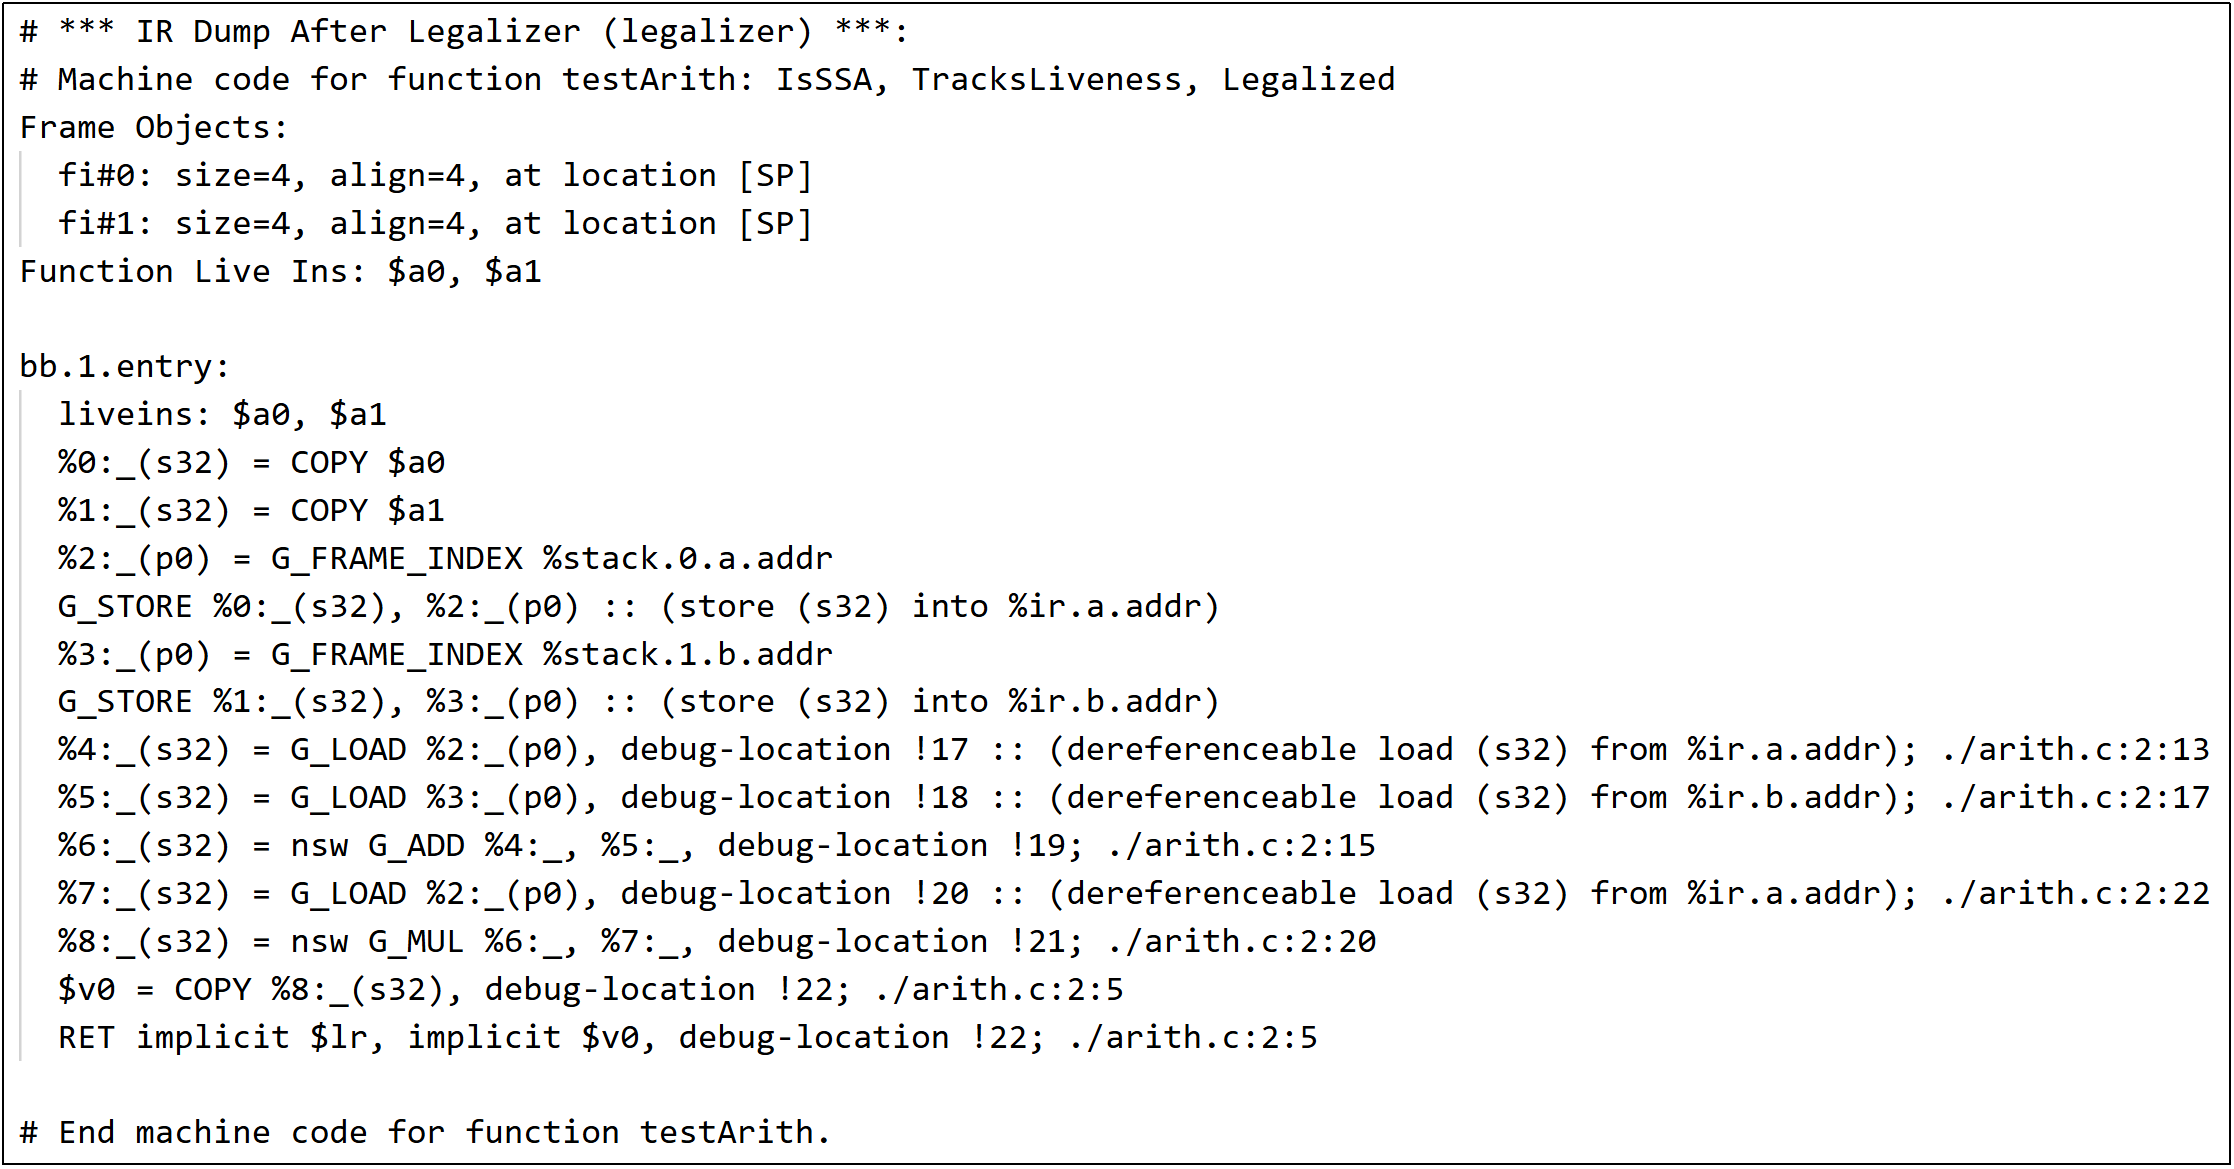
\includegraphics[width=1\textwidth]{pics/case_1_legalize_dump.png}
	\caption{示例一合法化阶段Dump图}
	\label{fig:case_1_legalize_dump}
\end{figure}

4.寄存器组选择阶段

在寄存器组选择阶段,编译器为每个虚拟寄存器分配合适的寄存器组。在DSP后端中,参与整数算术运算的虚拟寄存器统一映射至通用整数寄存器组GPRB。如图\ref{fig:case_1_regbank_select_dump}所示,从寄存器组选择后的Dump结果可以观察到,所有算术指令的操作数及结果均被分配到GPRB寄存器组,且寄存器类型与操作数位宽保持一致。

\begin{figure}[htbp]
	\centering
	\includegraphics[width=1\textwidth]{pics/case_1_regbank_select_dump.png}
	\caption{示例一寄存器组选择阶段Dump图}
	\label{fig:case_1_regbank_select_dump}
\end{figure}

该结果表明所有参与算术运算的虚拟寄存器均被正确分配至通用寄存器组,同时未引入额外的跨寄存器组数据复制或冗余中间指令。

5.机器指令选择阶段

在机器指令选择阶段,GMIR被转换为DSP架构的目标机器指令。如\ref{fig:case_1_instr_select_dump}所示,从Dump结果可以观察到所有中间指令(除COPY外,需要在后续Pass中单独处理)都被正确的映射到DSP后端机器指令。

\begin{figure}[htbp]
	\centering
	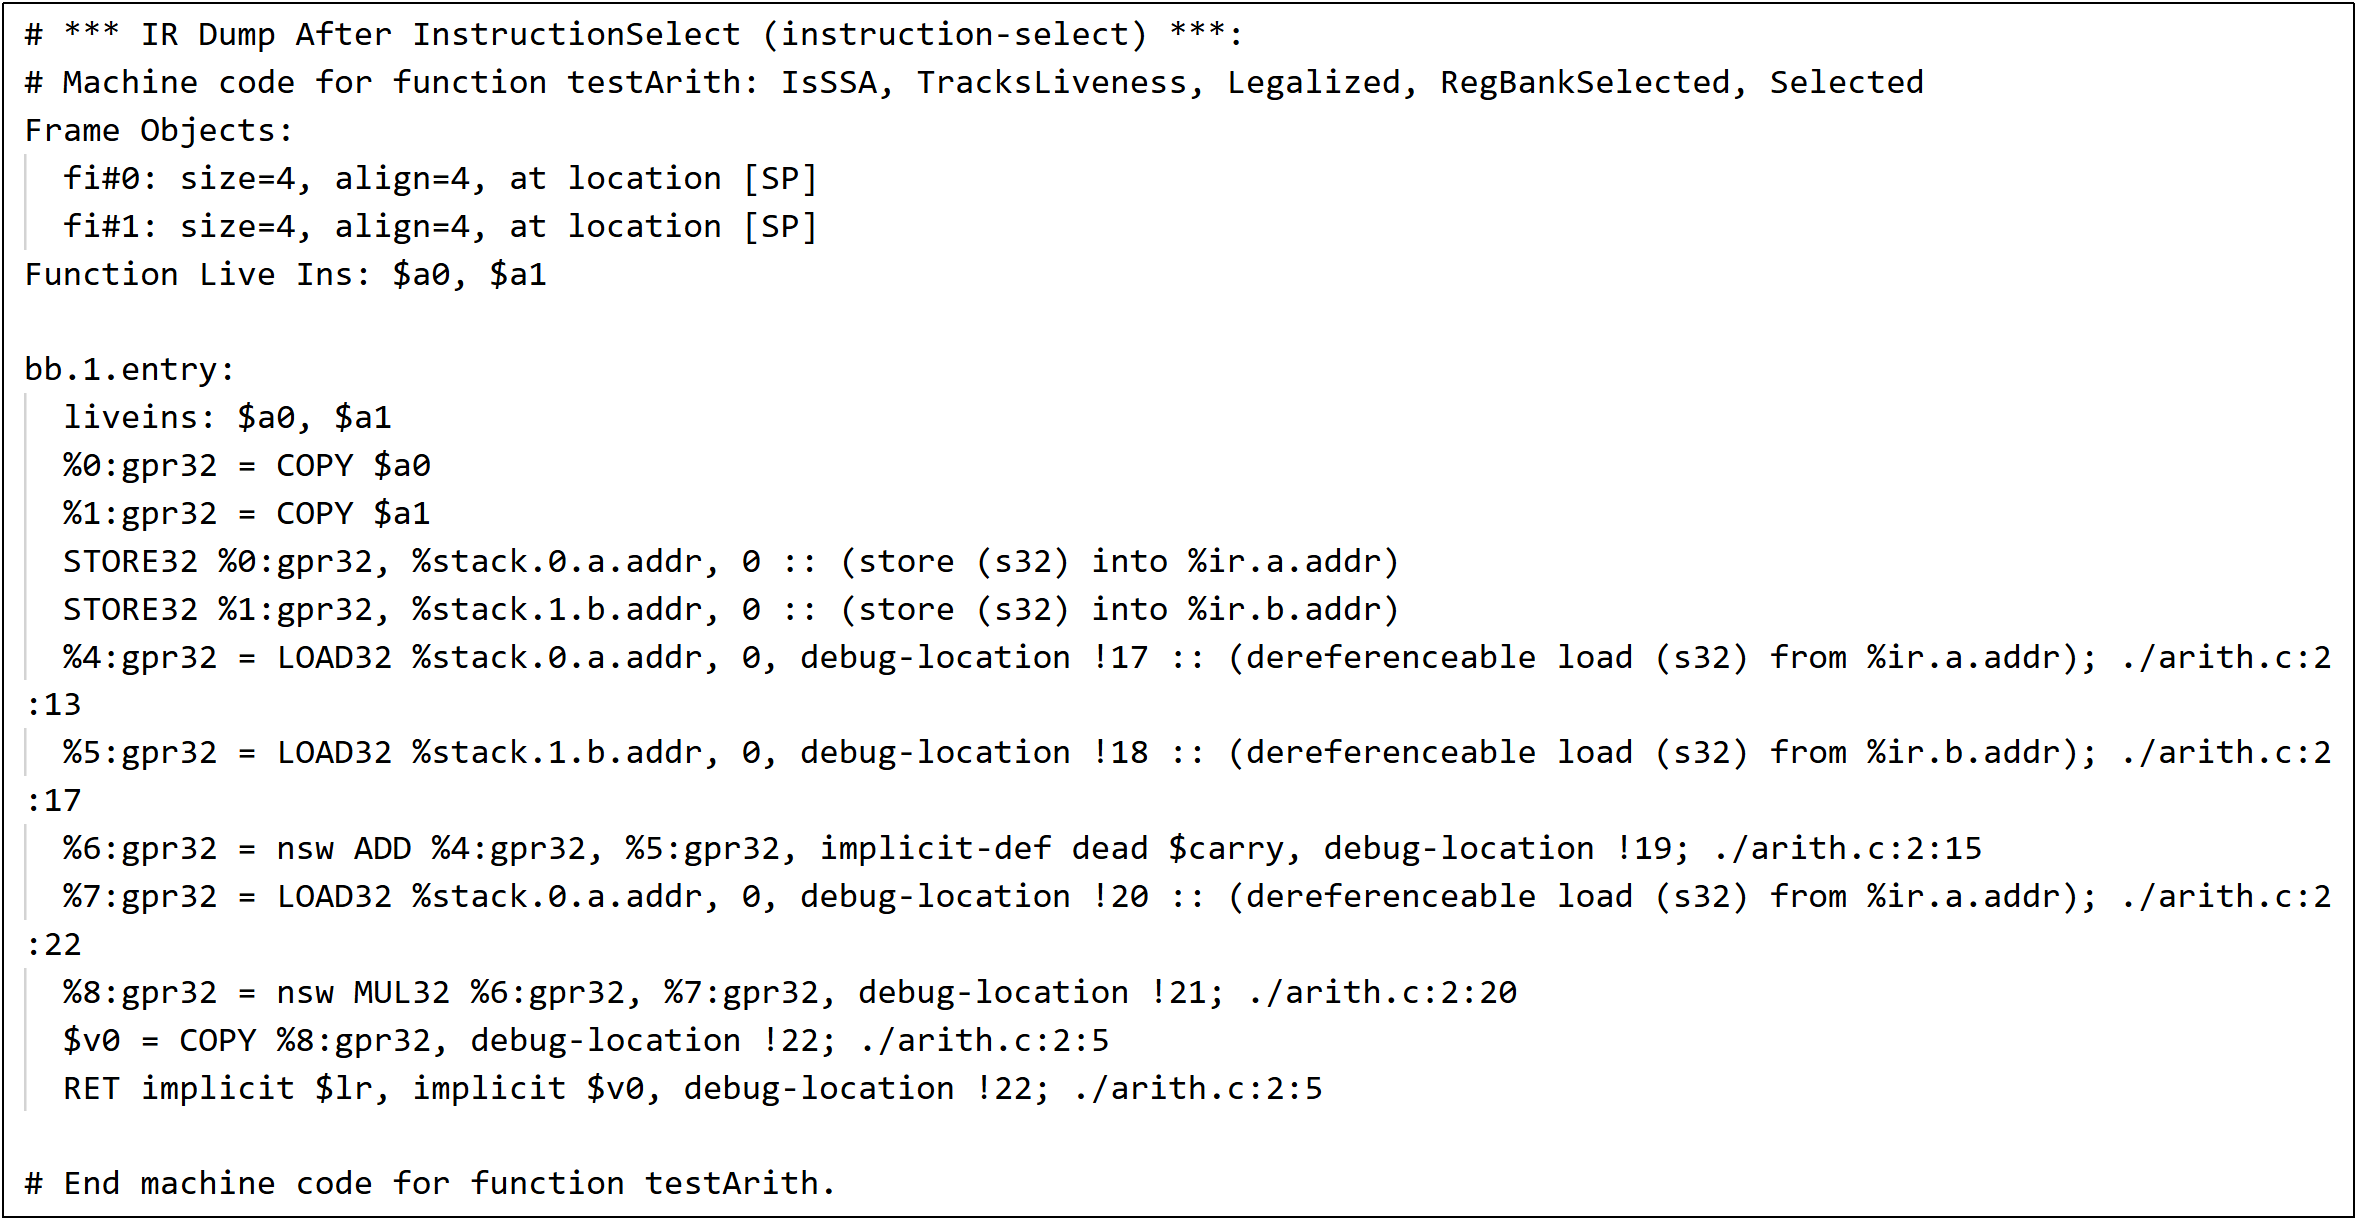
\includegraphics[width=1\textwidth]{pics/case_1_instr_select_dump.png}
	\caption{示例一机器指令选择阶段Dump图}
	\label{fig:case_1_instr_select_dump}
\end{figure}

6.最终代码生成

在经过寄存器分配、指令调度等后续后端Pass处理后,最终生成合法且可执行的DSP机器码。如图\ref{fig:case_1_final_dump}所示,整体代码生成流程未出现语义偏差或异常,验证了基本指令在GlobalISel框架下的端到端正确性。

\begin{figure}[htbp]
	\centering
	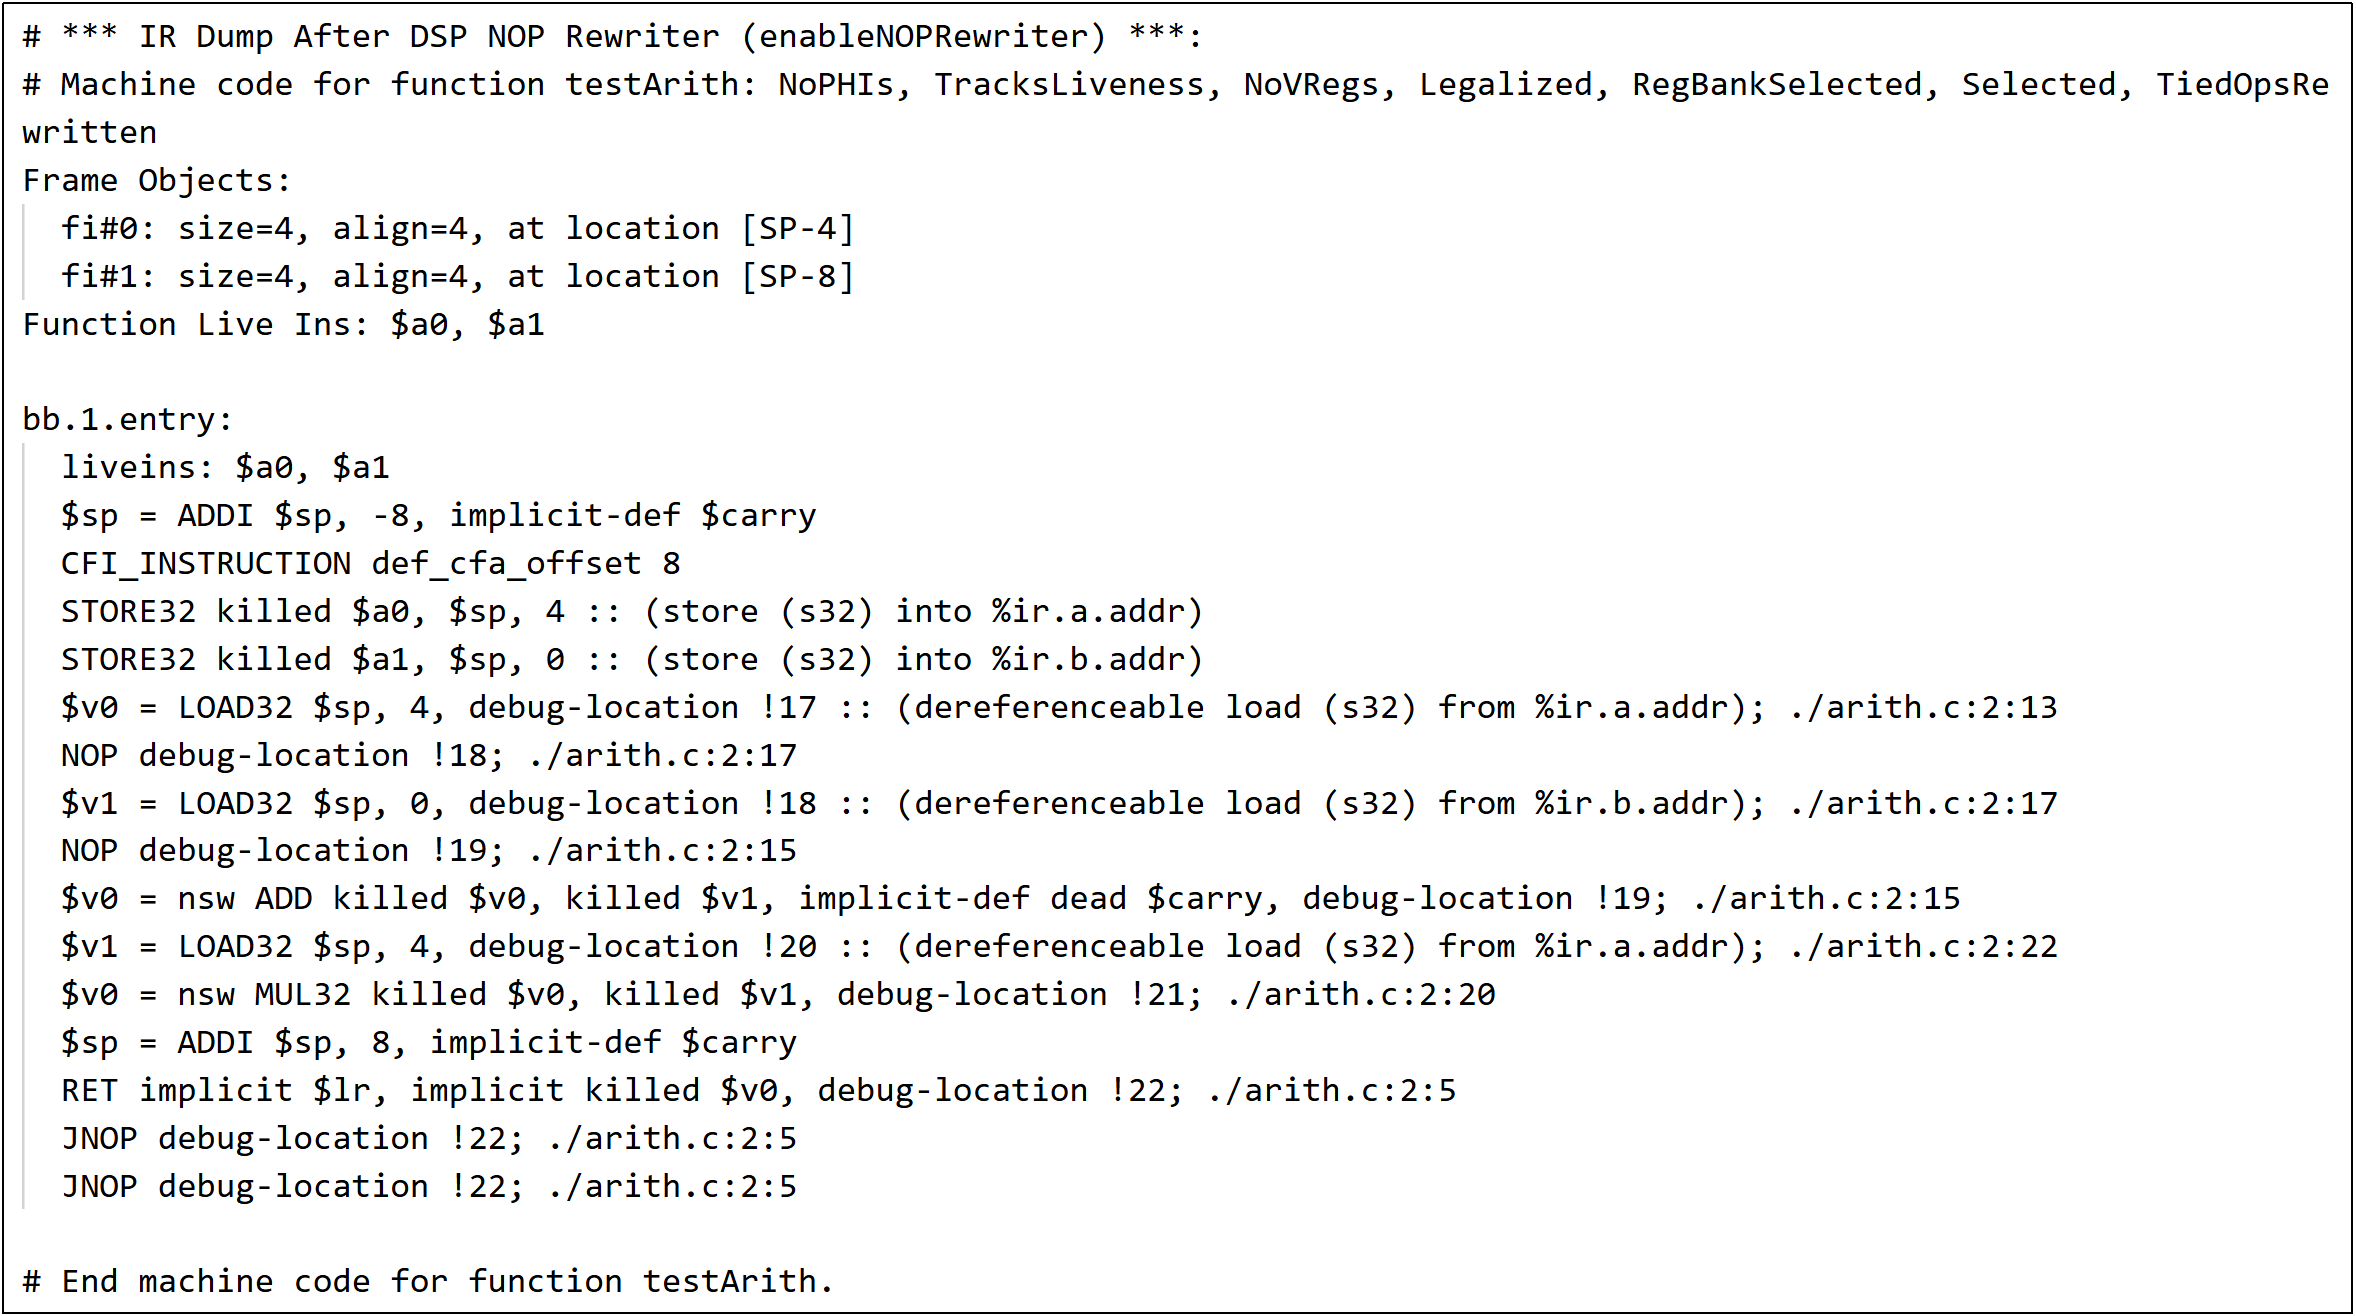
\includegraphics[width=1\textwidth]{pics/case_1_final_dump.png}
	\caption{示例一最后阶段Dump图}
	\label{fig:case_1_final_dump}
\end{figure}


% 5.1.2 控制流指令正确性验证
\subsection{控制流指令正确性验证}
除基本算术与内存访问指令这些基本指令外,控制流指令的正确生成和映射同样是验证编译器后端正确性的重要体现。本节针对对控制流相关指令的处理过程进行验证,重点覆盖比较与条件分支、循环结构以及函数调用三类典型控制流场景。

\par

1.比较+分支+跳转指令

比较与条件分支是程序控制流构建的基础。在LLVM IR中,该类操作通常通过icmp与br指令组合表达;在GlobalISel框架下,则对应为G\_ICMP与G\_BRCOND等GMIR指令。为验证DSP后端对该类控制流指令的处理正确性,本文构建了一个同时包含比较、条件分支及无条件跳转的示例二,其LLVM IR如下所示:

\lstset{language=c++}
\begin{lstlisting}
define dso_local i32 @testBranch() {
	entry:
	%retval = alloca i32
	%a = alloca i32
	%b = alloca i32
	store i32 10, ptr %a
	store i32 20, ptr %b
	%0 = load i32, ptr %a
	%1 = load i32, ptr %b
	%cmp = icmp slt i32 %0, %1
	br i1 %cmp, label %if.then, label %if.else
	
	if.then:
	store i32 0, ptr %retval
	br label %return
	
	if.else:
	store i32 1, ptr %retval
	br label %return
	
	return:  %2 = load i32, ptr %retval
	ret i32 %2
}
\end{lstlisting}

针对该示例,在GlobalISel各关键阶段中的处理过程如下:

\begin{itemize}
	\item
	在GMIR生成阶段,LLVM IR中的比较指令被正确转换为G\_ICMP,其比较谓词与操作数保持一致;条件跳转指令被转换为G\_BRCOND,并以比较结果作为分支条件。
	
	\item
	在合法化阶段,由于DSP架构支持整数比较操作,无需进一步拆分,相关指令保持原有结构。
	
	\item 
	在寄存器组选择阶段,编译器为比较操作及其结果所涉及的虚拟寄存器分配了合适的寄存器组,确保比较结果能够以符合DSP架构约定的方式参与后续控制流指令。
	
	\item 
	在机器指令选择阶段,G\_ICMP与后续的G\_BRCOND会被联合处理,映射为DSP架构下的比较指令与条件跳转指令,比较结果通过条件码寄存器传递,从而完成分支控制。
	
\end{itemize}

如图\ref{fig:case_2_final_dump}所示,在函数入口基本块中,比较指令首先生成条件码寄存器状态,随后通过条件跳转指令根据比较结果在两个后继基本块之间进行分支选择,验证了比较与条件分支指令的正确映射。

\begin{figure}[htbp]
	\centering
	\includegraphics[width=1\textwidth]{pics/case_2_final_dump.png}
	\caption{示例二入口基本块最后阶段Dump图}
	\label{fig:case_2_final_dump}
\end{figure}

如图\ref{fig:case_2_final_dump_2}所示,条件分支后的if.then与if.else基本块分别执行对应路径逻辑,并通过无条件跳转汇合至统一的返回基本块。最终生成的机器码中,各分支路径与返回块之间的控制流关系与LLVM IR描述保持一致。

\begin{figure}[htbp]
	\centering
	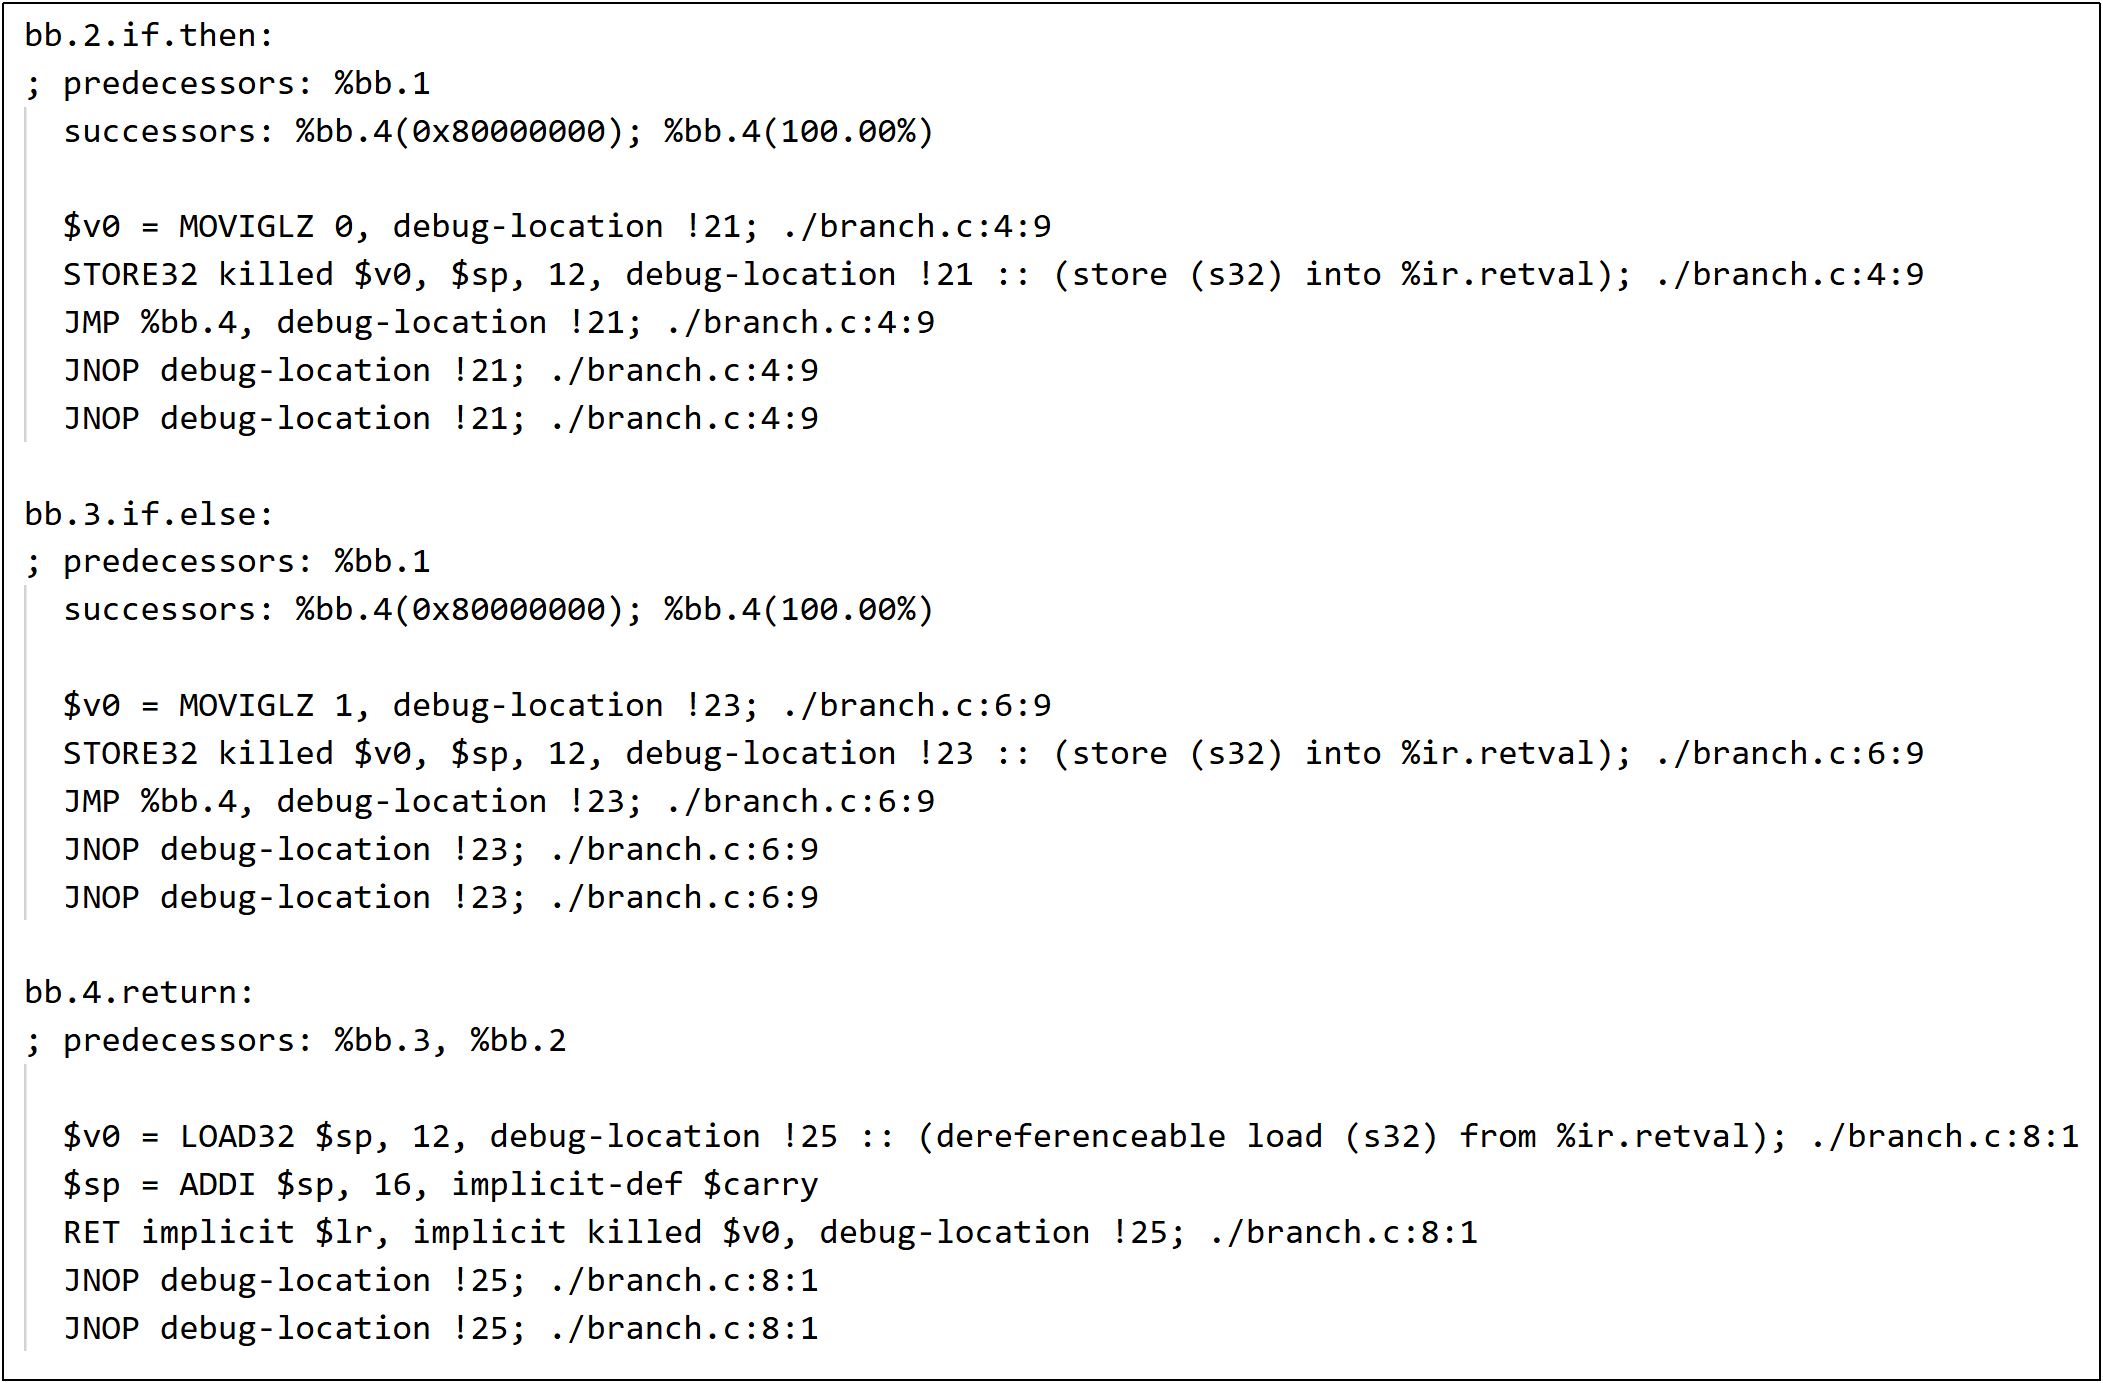
\includegraphics[width=1\textwidth]{pics/case_2_final_dump_2.png}
	\caption{示例二条件分支基本块最后阶段Dump图}
	\label{fig:case_2_final_dump_2}
\end{figure}

实验结果表明,从LLVM IR到最终机器码的转换过程中,比较条件与分支目标均保持一致,程序控制流未发生偏移或错误跳转,验证了比较与分支指令选择的正确性。

\par

2.循环指令

循环结构通常由条件判断、分支跳转以及回边构成,是控制流指令组合应用的典型场景。在LLVM IR中,循环通过多个基本块以及br指令共同表示;在GMIR层面,该多基本块结构及其控制流关系被完整保留下来,为后端代码生成提供了清晰的控制流语义。

\par

为验证DSP后端对循环指令的处理正确性,本文构建了一个包含循环指令的示例三,其LLVM IR如下所示:

\lstset{language=c++}
\begin{lstlisting}
define dso_local i32 @testLoop() {
	entry:
	%i = alloca i32
	store i32 0, ptr %i
	br label %for.cond
	
	for.cond:
	%0 = load i32, ptr %i
	%cmp = icmp slt i32 %0, 10
	br i1 %cmp, label %for.body, label %for.end
	
	for.body:
	br label %for.inc, !dbg !21
	
	for.inc:
	%1 = load i32, ptr %i
	%inc = add nsw i32 %1, 1
	store i32 %inc, ptr %i
	br label %for.cond
	
	for.end:
	ret i32 0
}
\end{lstlisting}

针对该示例,在GlobalISel各关键阶段中的处理过程如下:

\begin{itemize}
	\item
	在GMIR生成阶段,各基本块及其控制流关系被准确映射为MBB,循环条件与跳转关系通过G\_BR与G\_BRCOND指令表达。
	
	\item
	在合法化阶段,合法化前后指令结构保持一致,表明DSP后端的合法化规则能够覆盖该类循环场景的基本操作需求。
	
	\item 
	在寄存器组选择阶段,循环体内的算术与内存操作被正确映射至DSP通用寄存器组,循环条件判断所依赖的比较结果亦能够被正确传播。
	
	\item 
	在机器指令选择阶段,循环控制流相关的G\_ICMP与G\_BRCOND被联合分析并映射为DSP架构下的比较指令与条件跳转指令:比较结果通过条件码寄存器生成,并由条件跳转指令读取实现分支决策。
	
\end{itemize}

如图\ref{fig:case_3_final_dump}所示,在循环条件基本块中,编译器首先对循环变量与上界进行比较,并通过条件码寄存器生成分支条件,随后依据比较结果在循环体与循环结束块之间进行跳转,验证了循环条件判断与分支决策逻辑的正确性。

\begin{figure}[htbp]
	\centering
	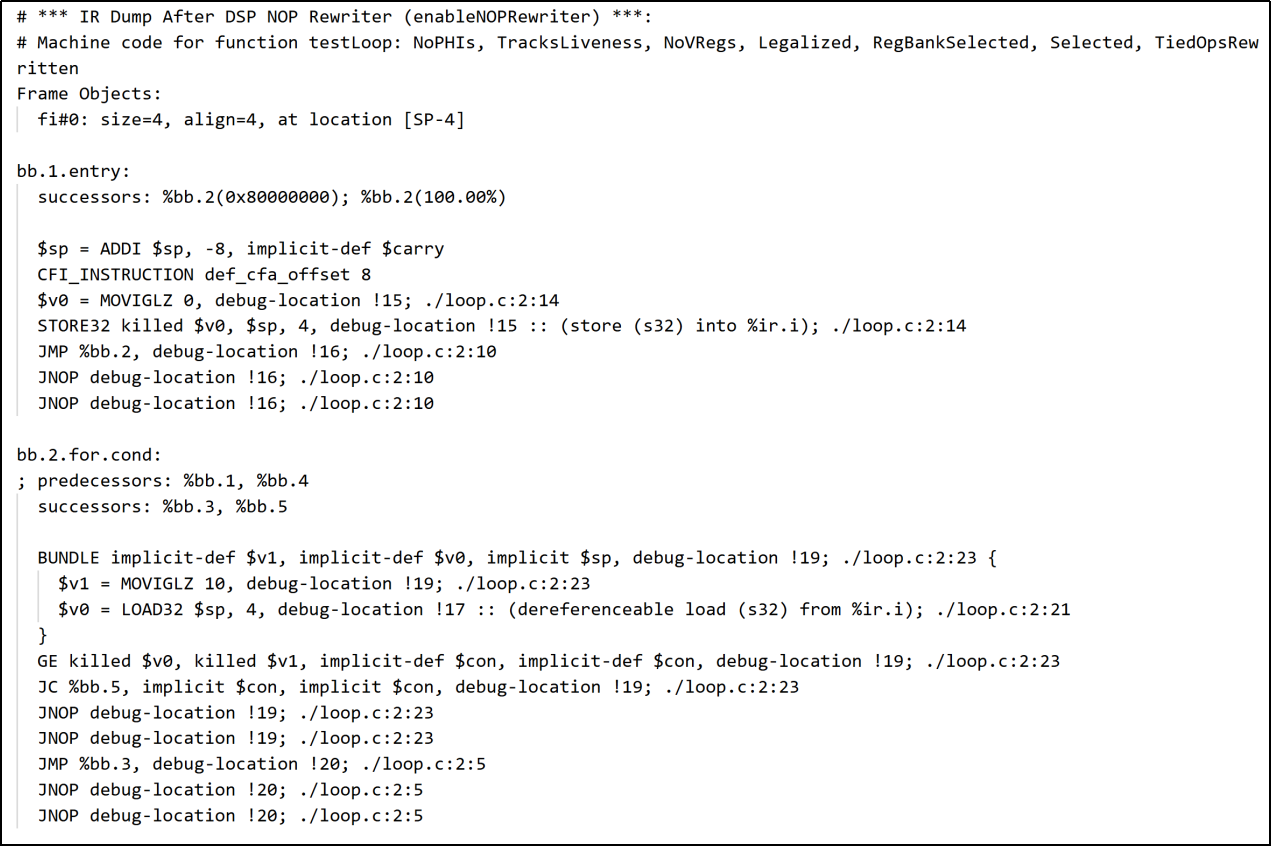
\includegraphics[width=1\textwidth]{pics/case_3_final_dump.png}
	\caption{示例三循环条件基本块最后阶段Dump图}
	\label{fig:case_3_final_dump}
\end{figure}


如图\ref{fig:case_3_final_dump_2}所示,循环体与自增基本块在执行完成后通过无条件跳转形成回边,并重新进入条件判断块;当循环条件不满足时,控制流正确跳转至循环结束块并完成函数返回,表明循环控制流在后端生成过程中保持一致。

\begin{figure}[htbp]
	\centering
	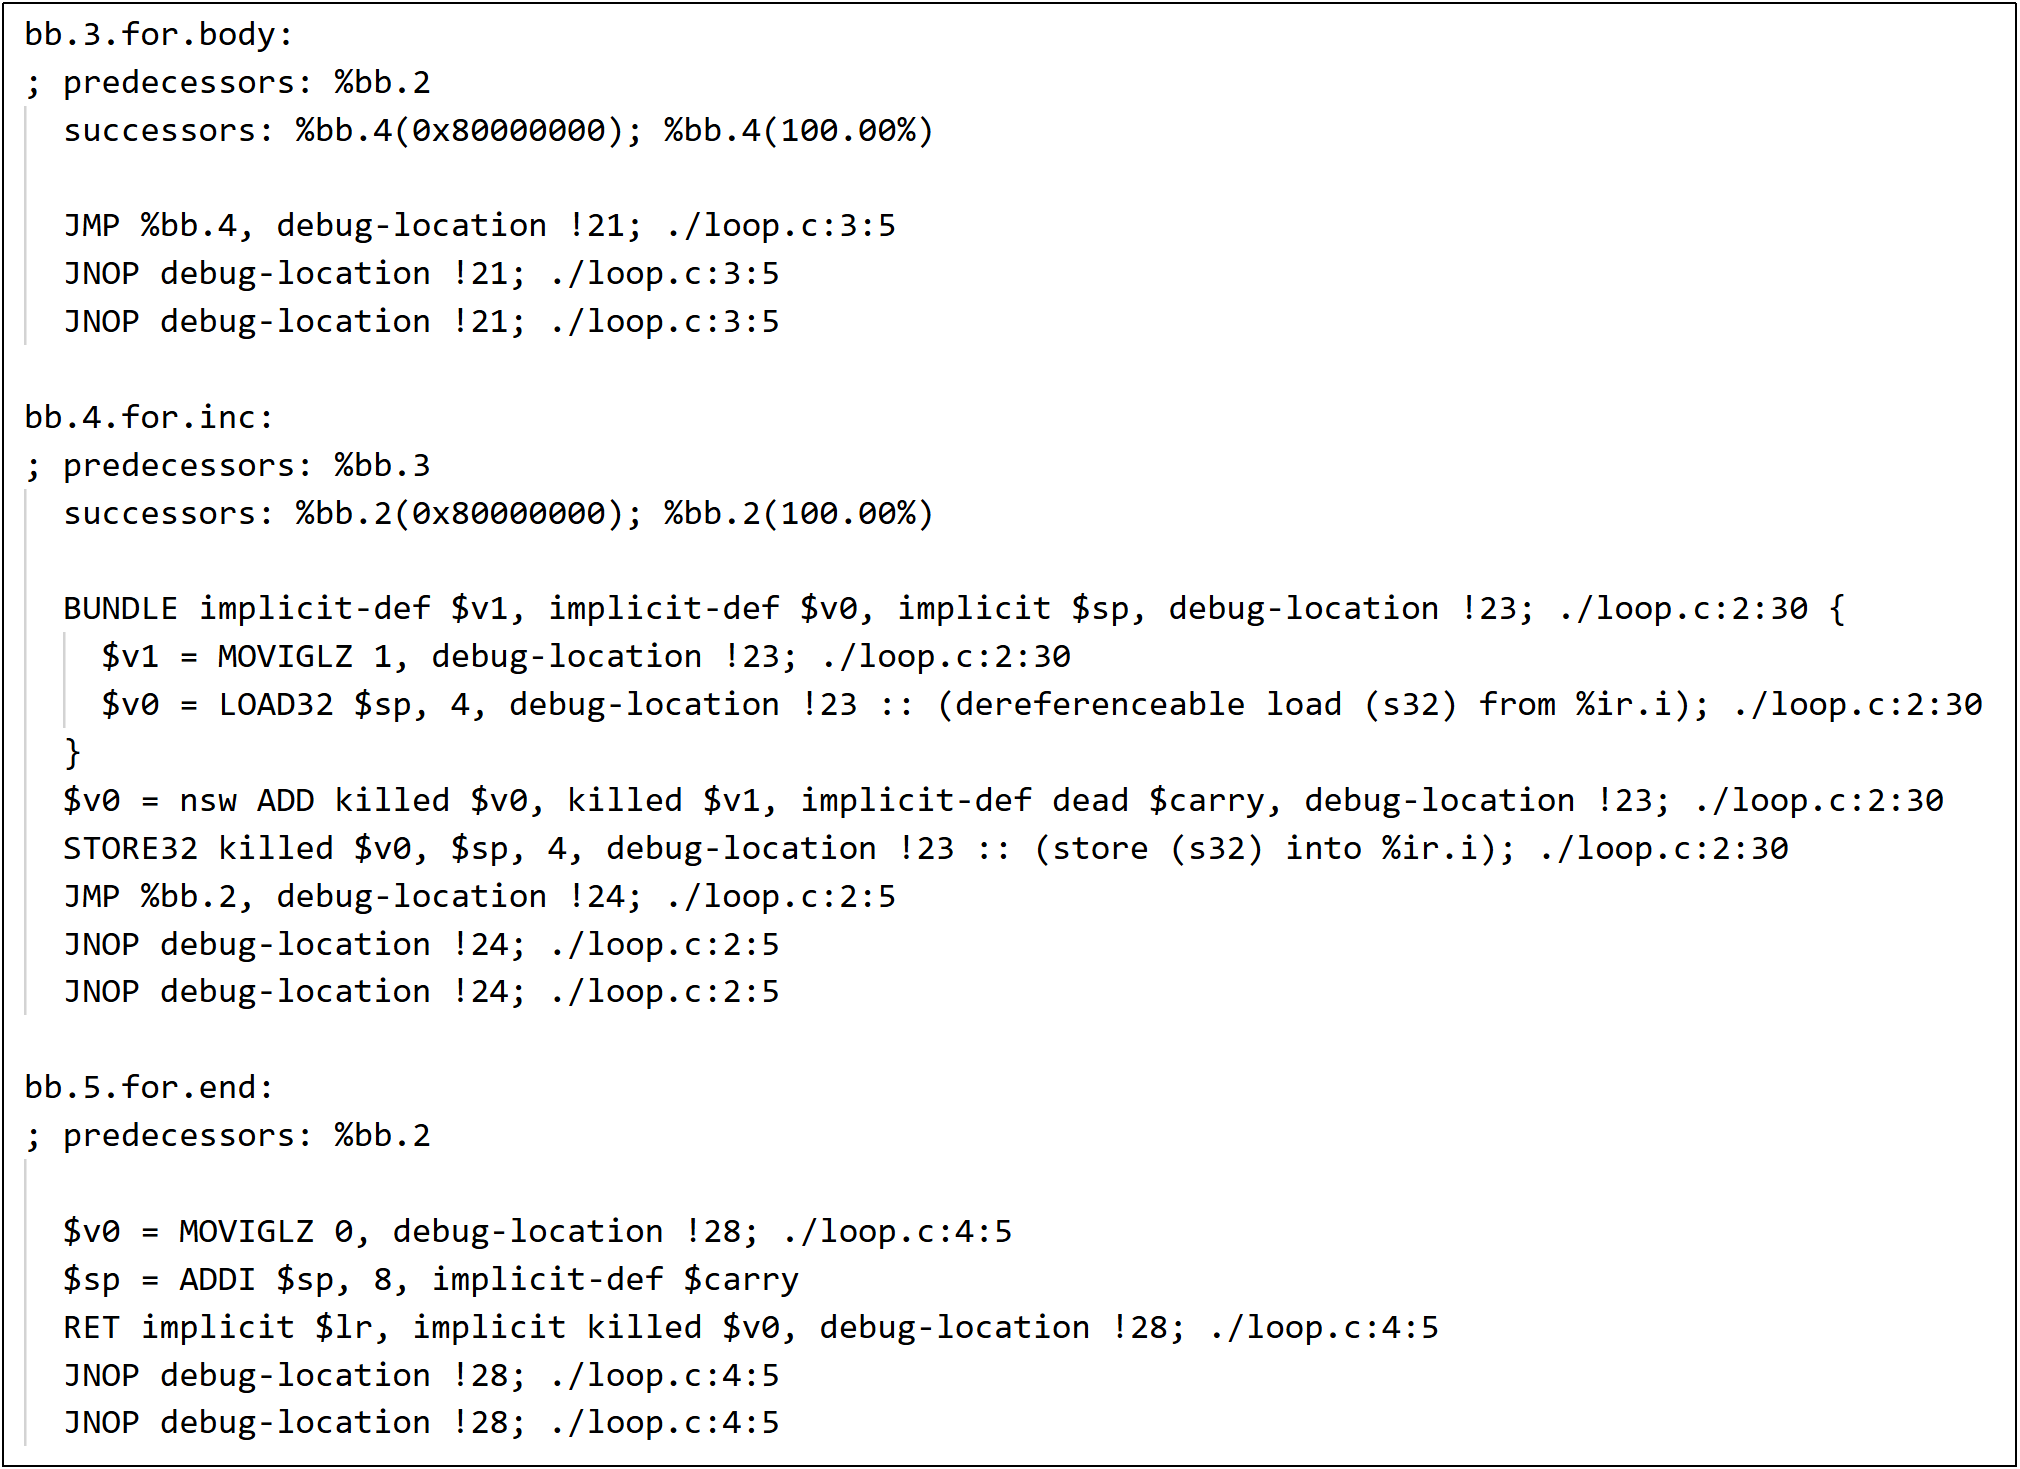
\includegraphics[width=1\textwidth]{pics/case_3_final_dump_2.png}
	\caption{示例三循环体基本块最后阶段Dump图}
	\label{fig:case_3_final_dump_2}
\end{figure}


从最终生成的机器码可以观察到,循环入口、循环体以及循环回边对应的跳转指令均与原始LLVM IR的控制流结构保持一致,且不存在多余或缺失的跳转指令。这表明GlobalISel在DSP后端中能够正确处理多基本块循环结构,确保循环语义的正确性。

\par

3.函数调用指令

函数调用是另一类重要的控制流操作,其正确性依赖于调用约定、参数传递以及返回值处理等多个方面。在LLVM IR中,函数调用通过call指令表示;在GlobalISel框架下,该过程涉及CallLowering与指令选择等多个阶段。

\par

为验证DSP后端在GlobalISel框架下对函数调用指令的处理正确性,构造了一个简单的示例四,其中main函数调用前文定义的testBranch函数,其LLVM IR如下所示:

针对该示例函数,函数调用在各阶段的处理过程如下:

\begin{itemize}
	\item
	在GMIR生成阶段,call指令被转换为一系列与调用约定相关的GMIR指令,包括参数准备、调用指令以及返回值接收等操作。
	
	\item
	在合法化阶段,合法化前后指令结构保持一致,表明DSP后端的合法化规则能够覆盖该类函数调用场景的基本操作需求。
	
	\item 
	在寄存器组选择阶段,函数参数与返回值被分配至DSP架构规定的寄存器或栈位置,符合DSP ABI的约定规则。
	
	\item 
	在机器指令选择阶段,调用相关的GMIR指令被映射为DSP架构支持的跳转与返回指令,并正确维护返回地址与调用现场。最终生成的机器码中,函数调用前后的寄存器状态与栈帧布局保持一致,函数返回值能够被正确读取并参与后续计算。
	
\end{itemize}

如图\ref{fig:case_4_final_dump}所示,实验结果表明DSP后端在GlobalISel框架下能够正确完成函数调用相关控制流的指令选择,保证跨函数控制流的正确传递。

\begin{figure}[htbp]
	\centering
	\includegraphics[width=1\textwidth]{pics/case_4_final_dump.png}
	\caption{示例四最后阶段Dump图}
	\label{fig:case_4_final_dump}
\end{figure}


%*********************************************************************
% 5.2 全局指令选择性能分析
%*********************************************************************
\section{全局指令选择性能分析}
本章主要针对编译时间、代码大小以及执行周期三个方面来对基于DAG的指令选择、未优化的全局指令选择以及优化的全局指令选择来进行对比。


% 5.2.1 编译时间
\subsection{编译时间}
编译时间的量化分析基于Clang自带的编译时间追踪功能实现,该机制能够对编译过程中各阶段的执行时间进行精细化统计,从而为分析编译器性能瓶颈与优化效果提供可靠的数据支撑。图\ref{fig:compile_time_example}中展示了部分关键时间指标及其在不同编译阶段的分布情况。

\begin{figure}[htbp]
	\centering
	\includegraphics[width=1\textwidth]{pics/compile_time_example.png}
	\caption{不同编译阶段时间指标图}
	\label{fig:compile_time_example}
\end{figure}

时间指标说明:

\begin{itemize}
	\item
	User Time(用户态时间):表示CPU在用户态执行编译器自身代码所消耗的时间,仅反映编译器逻辑计算的开销,不包含操作系统内核相关操作。
	
	\item
	System Time(系统态时间):表示CPU在内核态执行系统调用(如文件读写、内存管理、进程调度等)所消耗的时间,属于编译过程中的系统辅助开销。
	
	\item 
	User+System Time(用户态加系统态时间):反映CPU在该阶段用于计算的总耗时,是用户态和系统态时间的累加,但不包含I/O等待和CPU空闲时间。
	
	\item 
	Wall Time(壁钟时间):指从编译阶段开始到结束所经历的实际物理时间,包含CPU计算、I/O等待、进程调度以及资源竞争等所有因素。在真实工程场景中,该指标最能直观反映用户实际感知到的编译等待时长,因此也是本文关注的核心量化指标。
	
\end{itemize}

编译阶段划分:

\begin{itemize}
	\item
	Front end(前端):包括源代码解析、语法分析、语义分析等操作,主要负责将高级语言代码转换为中间表示。
	
	\item
	LLVM IR generation(LLVM IR生成):将前端分析结果转换为LLVM中间表示,为后续优化和代码生成奠定基础。
	
	\item 
	Optimizer(优化器):对LLVM IR进行多级优化,包括控制流优化、数据流优化及目标无关优化等。
	
	\item 
	Machine code generation(机器码生成):编译器后端的核心阶段,负责指令选择、寄存器分配、指令调度以及最终目标机器码的生成。
	
\end{itemize}

由于指令选择阶段在LLVM后端中与其他流程高度耦合,难以单独抽离并进行精确量化,因此本文在编译时间分析中,将关注点放在后端整体执行时间上。具体而言,仅统计Machine Code Generation阶段的Wall Time,以此作为后端编译开销的统一度量标准。该统计方式在保证分析结果可比性和稳定性的同时,能够有效反映后端相关优化对实际编译时间的影响,为后续性能评估提供依据。

\par

图\ref{fig:compile_time_contrast}给出了在Embench测试集上两种指令选择方案在不同优化等级下的平均编译时间对比结果。为降低单次测量中噪声和偶然因素对实验结果的影响,本文采用多次重复实验的统计方法:在相同实验环境与配置条件下,对每个测试样例分别执行10次编译;在结果统计阶段,剔除两个最大值和两个最小值,对剩余数据取平均值作为该样例在对应优化等级下的编译时间。随后,对Embench测试集中的22个基准程序的结果进一步取平均,得到图中所示的最终统计结果。该统计过程覆盖了四个优化等级,能够较为全面且稳定地反映不同指令选择方案在实际编译流程中的时间开销特征。

\begin{figure}[htbp]
	\centering
	\includegraphics[width=1\textwidth]{pics/compile_time_contrast.png}
	\caption{两种指令选择方案平均编译时间对比图}
	\label{fig:compile_time_contrast}
\end{figure}

从图中可以看出,在各优化等级下,两种指令选择方案在编译时间上表现出一定差异,其中GlobalISel在所有优化等级下都具有更低的平均编译时间,体现了其在指令选择阶段流程简化和整体编译效率方面的优势。


% 5.2.2 代码大小
\subsection{代码大小}





% 5.2.3 执行周期
\subsection{执行周期}






%*********************************************************************
% 5.3 测试评估平台展示
%*********************************************************************
\section{测试评估平台展示}
测试评估平台围绕编译器工具链的持续迭代需求进行设计,集成了性能数据采集、历史回归分析、版本对比以及汇编级诊断等功能。平台通过对不同Commit在统一测试集上的性能表现进行系统化记录与分析,已在实际开发过程中协助发现并定位多个影响性能或代码生成质量的工具链缺陷,为编译器优化与回归验证提供了重要支撑。下文结合平台主要功能界面,详细展示其核心功能。

\par

1.全局性能趋势分析

如图\ref{fig:summary}所示,界面用于展示历史Commit的整体性能概览,侧重于从宏观层面分析编译器性能随时间的演进趋势。该界面基于完整测试集,对不同Commit下的平均代码体积和平均执行周期进行统计与可视化展示,便于快速识别性能回退或异常波动,为后续深入分析提供依据;支持按测试集、测试平台以及芯片版本区分数据,同时展示测试集在不同优化等级及版本下的平均代码大小与平均执行周期。

\begin{figure}[htbp]
	\centering
	\includegraphics[width=1\textwidth]{pics/summary.png}
	\caption{全局性能趋势分析界面展示图}
	\label{fig:summary}
\end{figure}

2.单测试用例性能演化分析

如图\ref{fig:history}所示,界面用于跟踪单个测试用例在不同Commit下的性能变化情况,支持按时间序列展示其执行周期、代码大小以及指令打包效率等关键指标。通过该界面,开发者可以精确定位某一性能变化首次引入的Commit,从而显著提升性能回归分析的效率与准确性。

\begin{figure}[htbp]
	\centering
	\includegraphics[width=1\textwidth]{pics/history.png}
	\caption{单测试用例性能演化分析界面展示图}
	\label{fig:history}
\end{figure}


3.跨版本性能差异对比分析

如图\ref{fig:compare}所示,界面用于对任意两个Commit之间的性能指标进行对比分析。该界面不仅提供测试用例级别的执行周期与代码体积对比结果,还支持对生成的汇编代码进行逐行对照,帮助开发者从底层代码生成角度分析性能差异的根本原因,适用于优化效果验证与回归问题定位。

\begin{figure}[htbp]
	\centering
	\includegraphics[width=1\textwidth]{pics/compare.png}
	\caption{跨版本性能差异对比分析界面展示图}
	\label{fig:compare}
\end{figure}

4.本地性能测试报告上传

如图\ref{fig:custom}所示,界面用于上传本地生成的性能测试结果,并与Master分支的结果进行对比分析。该功能为开发者在本地修改编译器或新增优化策略后,快速验证其性能影响提供了便利,有效支持离线实验与在线结果的统一管理。

\begin{figure}[htbp]
	\centering
	\includegraphics[width=1\textwidth]{pics/custom.png}
	\caption{本地性能测试报告上传界面展示图}
	\label{fig:custom}
\end{figure}





